\documentclass[10pt]{article}
\usepackage{graphicx}
\usepackage{xeCJK}
\usepackage{placeins}
\usepackage{float}
\usepackage{amssymb}
\usepackage{amsmath}
\setCJKmainfont{MS Mincho} % for \rmfamily
\setCJKsansfont{MS Gothic} % for \sffamily
\graphicspath{ {../image/} }
\renewcommand{\figurename}{図}
\renewcommand{\tablename}{表}

\title{Assignment 1}

\author{Phusaeng Natthaphat (04B23054)}
\date{2026年4月27日}


\begin{document}
\maketitle

\section{課題}
\subsection{課題1}
　rand$()$関数を使って、Monte Carlo積分する。(Please see \texttt{pi\_hw\_rand.cpp})

\subsection{課題2}
　rand$()$ 関数の代わりにMersene Twister (MT) Algorithm を使う。(Please see \texttt{pi\_hw\_MT.cpp})

\subsection{結果}
　両方の方法を比較し、グラフにする。また、誤差$\delta(n)$も評価する。図\ref{fig:pi_montecarlo}から分かるように、
誤差は以下の関係を持つ。
\begin{equation}
    \delta(n)\sim \frac{1}{\sqrt{n}}
\end{equation}

\begin{figure}[H]
    \centering
    \makebox[\textwidth][c]{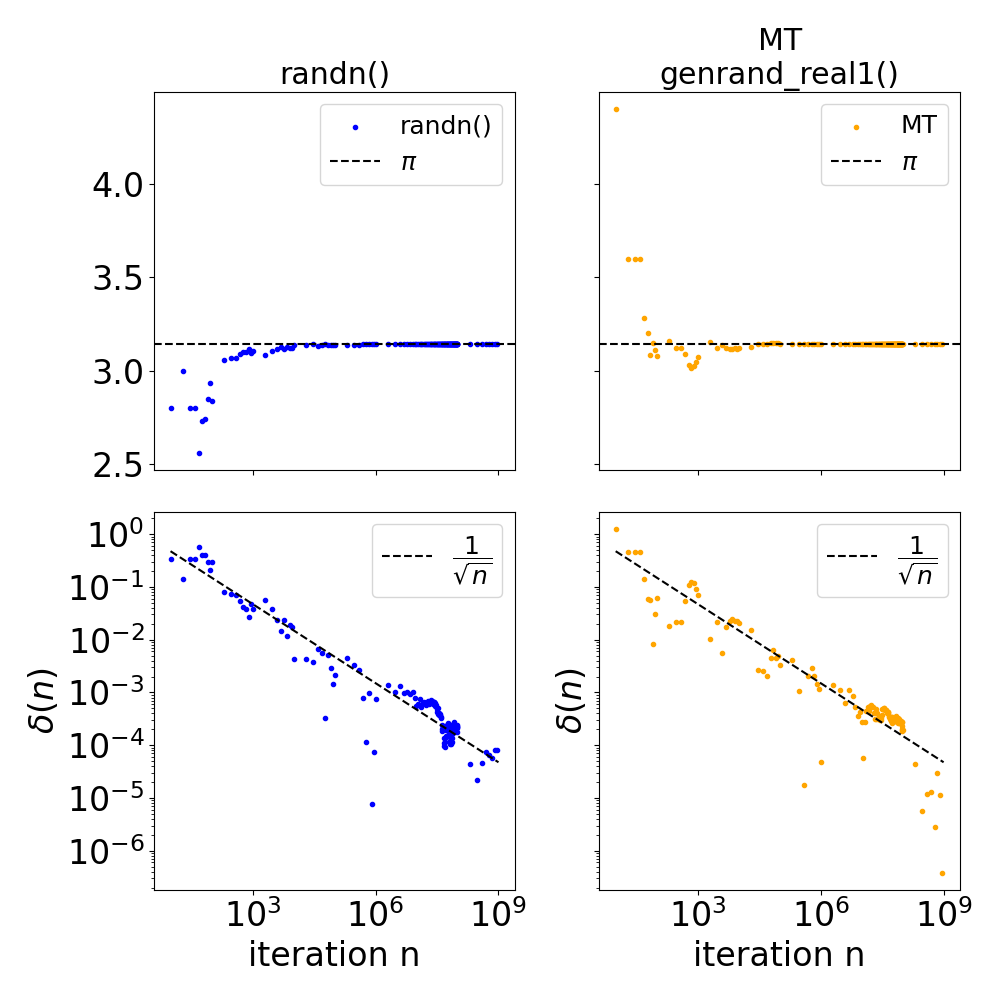
\includegraphics[width=\paperwidth]{MonteCarlo_pi.png}}
    \caption{$\pi$ from Monte Carlo Integration}
    \label{fig:pi_montecarlo}
\end{figure}
\section{考察}
\subsection{Monte Carlo Integration}
以下の積分を評価したい
\begin{equation}
    A = \int_{a}^{b}g(x)dx
\end{equation}
[a,b]上のi.i.d r.v. $\{X_i\}_{i\in\Lambda}$の密度関数は$f(x)$とし、
これらを用いて
\begin{equation}
    \tilde{A}(N):=\frac{1}{N}\sum_{i=1}^{N}\frac{g(X_i)}{f(X_i)}
\end{equation}
とおく。$\tilde{A}(N)$は$A$を推定するパラメータとなる。
\begin{equation}
    \begin{split}
        \mathbb{E}[\tilde{A}]   &=\frac{b-a}{N}N\int_{a}^{b}\frac{g(x)}{f(x)}f(x)dx\\
        &=\int_{a}^{b}g(x)dx\\
        &=A
    \end{split}
\end{equation}
$g(X_i)/f(X_i)$を新しい i.i.d. r.v. $Y_i$にしておく。すると
\begin{equation}
    \begin{split}
        \mathbb{V}[\tilde{A}]&=\mathbb{E}[(\tilde{A}-\mathbb{E}[\tilde{A}])^2]=\mathbb{E}[(\tilde{A}-A)^2]\\
        &:=\sigma^2
    \end{split}
\end{equation}
$\tilde{A}$の分散を$\sigma^2$におこう。\\
　中心極限定理(CLT)より、
\begin{equation}
    \lim_{N\rightarrow\infty}\tilde{A}\rightarrow \mathcal{N}(A,\frac{\sigma^2}{N})
\end{equation}
$\tilde{A}$は平均$\mathbb{E}[\tilde{A}]=A$、分散$\sigma^2/N$の正規分布に収束する。
誤差$\delta(N)$を次のように
\begin{equation}
    \delta(N)=|\tilde{A}(N)-A|=\sqrt{(\tilde{A}(N)-A)^2}
\end{equation}
定義する。すると$\delta^2(N)$の期待値は$\mathbb{V}[\tilde{A}]$で記述でき、実際にsimulationした$\delta'$は
\begin{equation}
    \delta':=\sqrt{\mathbb{E}[\delta^2]}=\sqrt{\mathbb{V}[\tilde{A}]}\rightarrow\frac{\sigma}{\sqrt{N}}
\end{equation}
$1/\sqrt{N}$に比例することが分かった。
\begin{enumerate}
    \item i.i.d は求められているが、$X_i$の分布は特に特定しない。つまり、どんな$X_i$を使っても同じ収束スピード$(\sim1/\sqrt{N})$になるはず
\end{enumerate}
\end{document}